\section{Presentación del Sistema de Gestión de PQRs}

El Sistema de Gestión de PQRs para el IDU es una extensión del módulo Office Of Citizen Services (Oficina de Atencion al Ciudadano) disponible 
en la plataforma de Software Libre OpenERP, 
el objetivo de este sistema es el de brindar a las organizaciones públicas que están obligadas a 
atender solicitudes de la ciudadanía una herramienta que permita registrar las PQR que ingresan por los diferentes canales y manejar su ciclo de vida
dentro de la organización, desde la creación hasta la finalización de la PQR donde se da la respuesta al ciudadano.\\
Adicionalmente, se incluye un componente de georeferenciación, que permite que la información 
sea consultada desde un Sistema de Información Geográfica como Quantum o gvSIG, esta característica permite realizar análisis geográficos de las PQRs registradas.\\

\subsection{Funcionalidad e integración con otros sistemas}

\begin{figure}[h]
 \centering6
 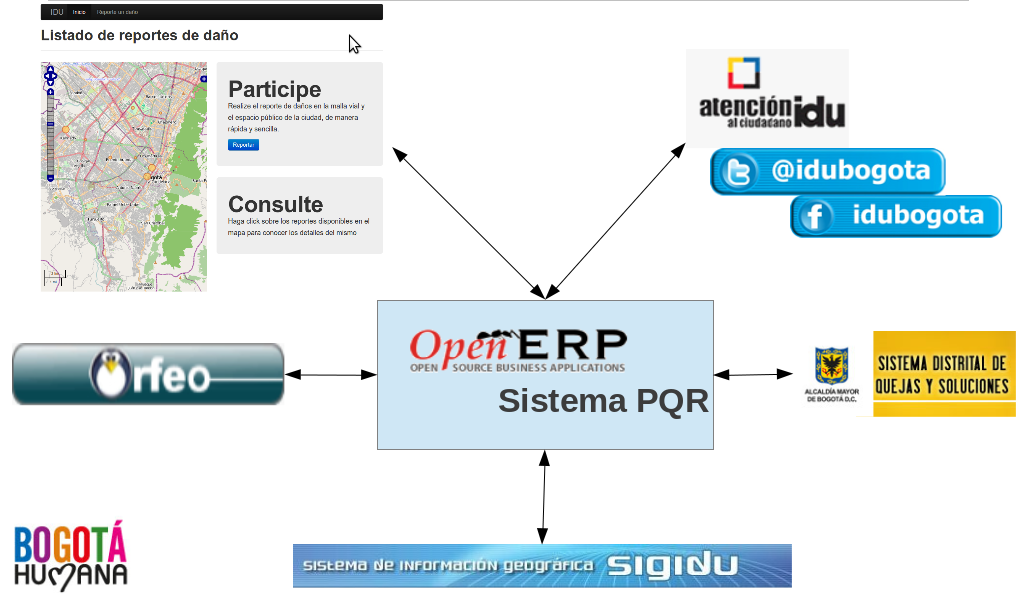
\includegraphics[width=17cm,height=9.5cm]{./Imagenes/slidesistemacompleto.png}
 % Login.png: 1289x610 pixel, 96dpi, 34.10x16.14 cm, bb=0 0 967 457
 \caption{Perspectiva actual del sistema OpenERP dentro del IDU}
 \label{fig:slidesistemacompleto}
\end{figure}

Al interior del IDU el sistema de PQRs se integra a los demás sistemas de información tal como se ve en la figura \ref{fig:slidesistemacompleto}. OpenERP consolida la 
información de todas las PQR que ingresan al instituto por los diversos canales. A su vez cuenta con los mecanismos para comunicarse con los otros sistemas de información 
relacionados: Sistema de Información Geográfico del IDU (SIGIDU), Sistema de Gestión Documental (Orfeo GPL), Sistema Distrital de 
Quejas y Soluciones (SDQS).\\

Las PQRs se tramitan de la siguiente manera: Se registran en OpenERP, allí son gestionadas por la Oficina de atención al ciudadano,
si no se cuenta con una respuesta inmediata, pasan a la dependencia relacionada de la organización a través del
sistema de Gestión Documental Orfeo, OpenERP espera la respuesta y conserva el número de radicación de Orfeo. Los casos y los documentos, son copiados también 
a SDQS, lo cual es necesario para cumplir la normativa Distrital.\\

El ciudadano dispone de una herramienta para registrar su PQR desde el portal Web Institucional, se trata del portal de Huecos,
desde ahí se diligencia un formulario con toda la información relacionada a los daños de la malla vial, se hace una clasificación y se ubica el 
punto en el mapa de la ciudad. El reporte es almacenado en OpenERP y luego tramitado.(Esta funcionalidad se encuentra en desarrollo)\\

Si un ciudadano llega personalmente a las instalaciones del IDU y radica un documento, este es digitalizado, ingresa al sistema Orfeo, si el 
documento se cataloga como una PQR, pasa automáticamente a OpenERP para que sea tramitado.(Esta funcionalidad se encuentra en desarrollo)\\

Si el ciudadano ingresa a la página de Internet de SDQS y crea una petición, esta es remitida al IDU por servicios Web, ingresa directamente a OpenERP, 
y allí se inicia el trámite correspondiente.(Esta funcionalidad se encuentra en desarrollo)\\

